\section{Introduction}

Telecommunication  infrastructures consist of a myriad of technologies from specialized domains such as radio,  access, transport, core and (virtualized) data center networks. Designing, deploying and operating end-to-end services are commonly   manual and long processes performed via traditional \gls{oss} resulting in long lead times (weeks or months) until effective service delivery~\cite{BluePlanet2017ProductsOrchestration}. Moreover, the involved workflows are commonly hampered by built-in hazards of infrastructures strongly coupled to physical topologies and hardware-specific constraints.

\begin{figure}[t!]
  \centering
  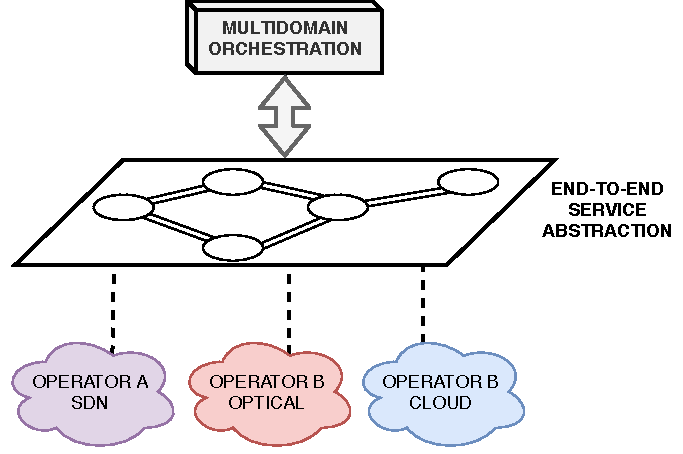
\includegraphics[scale=.75]{Figures/01_Introduction/intro}
    \caption{Context and scope of Network Service Orchestration.}
    \label{intro}
\end{figure}


Technological advances under the flags of \gls{sdn} \cite{surveySDN} and \gls{nfv} \cite{Mijumbi2016NetworkChallenges} bring new ways in which network operators can create, deploy, and manage their services. \gls{sdn} and \gls{nfv}, as well cloud computing introduce new means for efficient and flexible utilization of their infrastructures through a software-centric service paradigm \cite{Sonkoly2014UNIFYingView}. However, to realize this paradigm, there is a need to model the end-to-end service and have the ability to abstract and automate the control of physical and virtual resources delivering the service. The coordinated set of activities behind such process is commonly referred to as \textit{orchestration}. In general, orchestration refers to the idea of automatically selecting and controlling multiple resources, services, and systems to meet certain objectives (e.g., a customer requesting a specific network service). Altogether, the process shall be timely, consistent, secure, and lead to cost reduction due to automation and virtualization. We refer to \gls{nso} as the automated management and control processes involved in services deployment and operations  performed mainly by telecommunication operators and service providers, involving different types of resources and potentially multiple providers, as illustrated in Figure~\ref{intro}.



\begin{figure*}[t!]
  \centering
  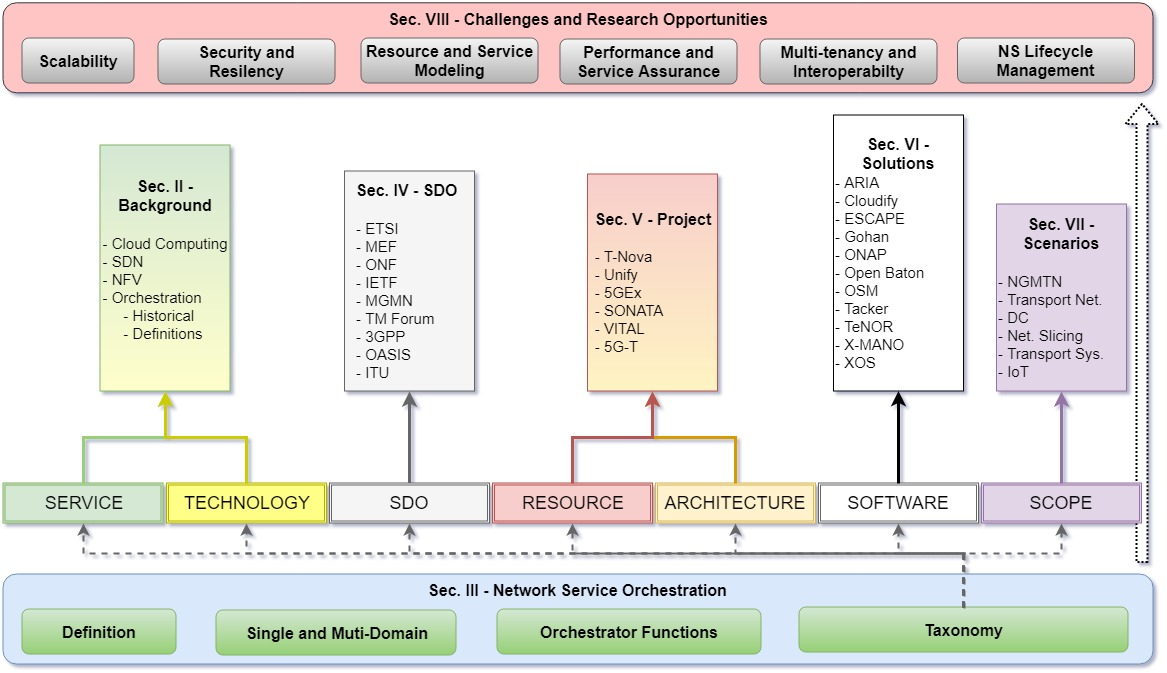
\includegraphics[scale=.6]{Figures/01_Introduction/org}
    \caption{Overview of the organization of this survey on NSO.}
    \label{org}
\end{figure*}

\gls{nso} is responsible for decoupling the high-level service layer (e.g., applications, service  slices, \gls{oss}) from the underlying management and resources layers (e.g., controllers, \gls{ems}, \gls{vim}), providing agility, enabling innovative service, optimizing resources, and altogether delivering a more flexible infrastructure for tailored services delivery. To this end, \gls{nso}  defines the interaction with (chains of) network functions in underlying technologies and infrastructures through adequate abstractions and a unifying pane glass for service definition and operation. For example, NSO may connect traditional OSS/BSS to network functions running in virtualized infrastructures. As depicted by the hourglass shape in Figure~\ref{orch}, the  significance of NSO as the inter-working glue resembles IP in the network protocol stack. %Besides, \gls{nso} gives service providers further control of their network services and enables developers to create new services and functions.  


\begin{figure}[t!]
  \centering
  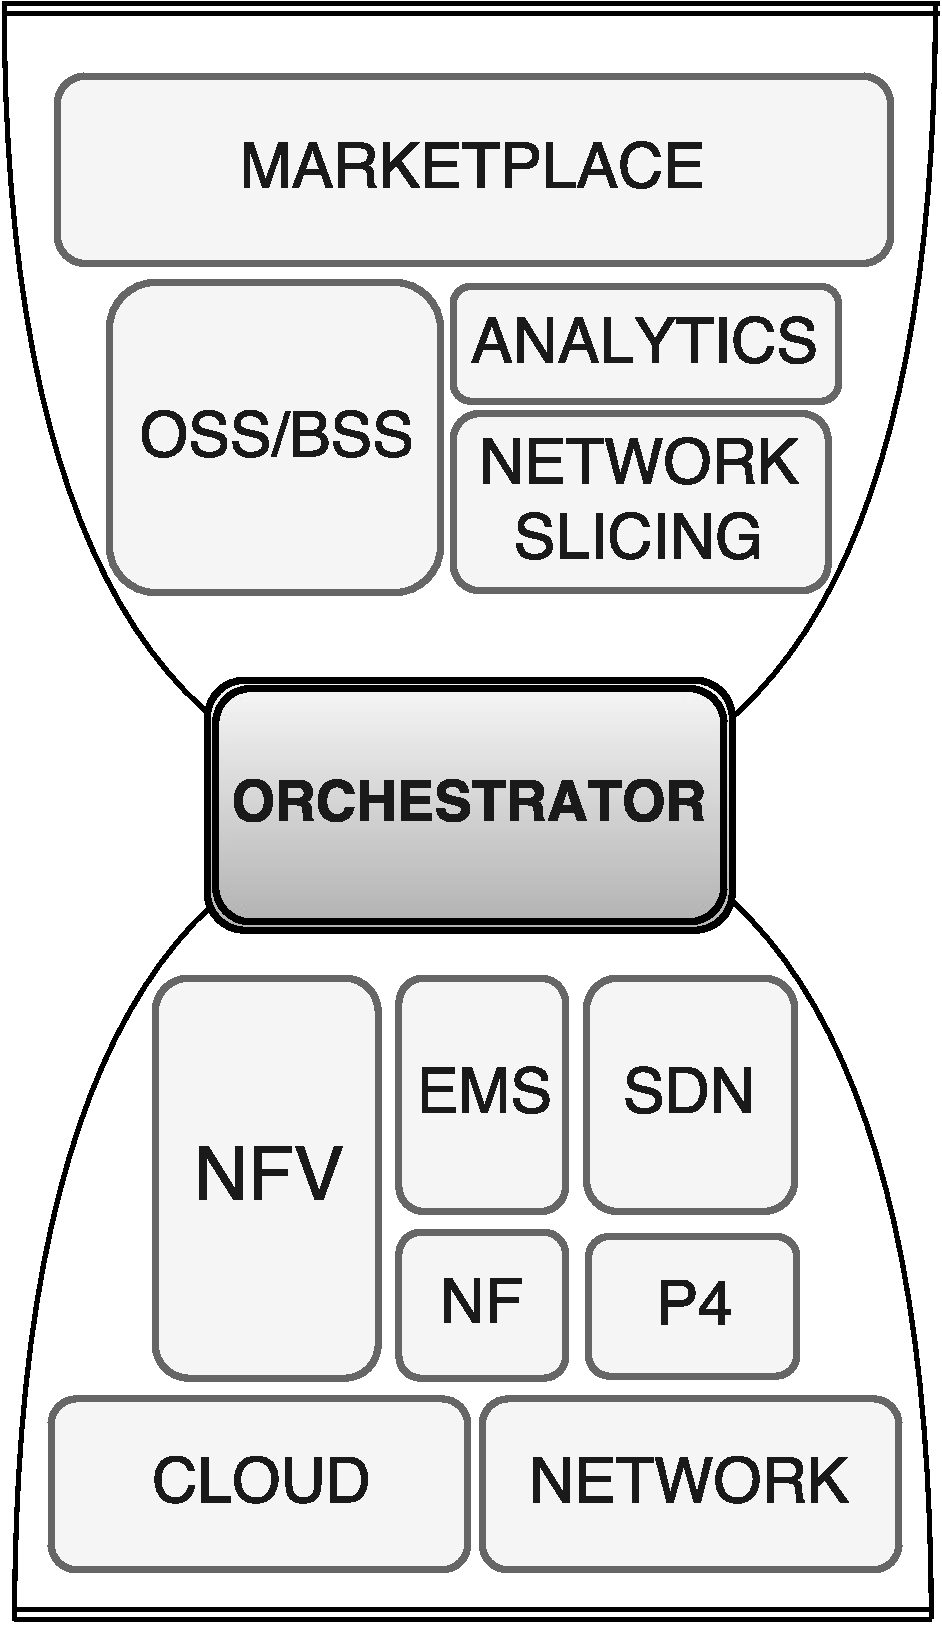
\includegraphics[scale=.2]{Figures/01_Introduction/orchestrator.pdf}
    \caption{Strategic role of the \gls{nso} as the glue between the actual services and the underlying management of resources.}
    \label{orch}
\end{figure}

As today, broad understanding and practical definitions of \gls{nso} are still missing -- not only across but also inside networking communities. The maturity of ongoing efforts varies largely with the overall technical approach being very much fragmented and showing little consolidation around an overarching notion of network service orchestration. %Generally, its scope is associated to network evolution.  

%%%%%% The orchestration and management piece is a higher layer which can glue the network, NFV, and many other pieces all together to create an automated business-driven platform. Orchestration and virtual management platform interact with the network control layer to create and provision the networking requirements, such as policies, network slices, traffic redirection, and service insertion for workloads. Source: EdX Course %%%%%%

%Many stakeholders are involved in the development and standardization of enabling technologies for network softwarization and their embodiment into next generation networks (e.g. 5G). The ecosystem includes \glspl{sdo}, as well as industry groups, open source projects, foundations, diverse user-lead groups, and so on. Examples of these players include \gls{etsi}, \gls{mef}, \gls{oasis}, Linux Foundation, and \gls{onf}. Similarly, in recent years, many (academic and industrial) research and (commercial) development efforts in orchestration, SDN and NFV have been concretized in a number of collaborative endeavors, for instance \gls{osm}~\cite{ETSIOpenMANO}, OpenStack~\cite{Foundationb}, \gls{onap}~\cite{onap}, \gls{5gex}~\cite{Guerzoni2016}, \gls{cord}~\cite{ON.LABOpenCORD}, etc.

%%%%%% ENHANCE
The main objective of this survey is to provide a comprehensive understanding of the research, standardization, and software development efforts around the overcharged term of  \acrlong{nso}. We present an in-depth and up-to-date study on network service orchestration covering some historical background and context, enabling technologies, standardization activities, actual solutions, open challenges, and research opportunities. We propose a taxonomy of the main characteristics and features of NSO approaches. We also make the mapping of the \gls{nso} primary characteristics and technical implementations to current open source platforms and research projects.    

Throughout the survey, we distinguish between two types of domains. First, \textit{administrative domains}, which map to different organizations and therefore may exist within a single service provider or cover a set of service providers. In one administrative domain, multiple \textit{technology domains} can exist based on the type of technology in scope, for example, Cloud, \gls{sdn}, \gls{nfv}, or Legacy. 
Broadly speaking, we refer to \gls{nso} as the automated coordination of resources and services embracing both single-domain and multi-domain footprints.  
%Network service orchestration aims at addressing operational hazards of service providers.

Figure~\ref{mdo} presents a generic high-level reference model for multi-domain Network Service Orchestration, featuring a \gls{mdo} per administrative realm and including the notion of a Marketplace for business interactions. 
\glspl{mdo} coordinate resources and services in a multiple administrative domain scope covering multiple technology domains~\cite{5GPPPArchitectureWorkingGroup2016ViewArchitecture}. 
The exchange of information, resources, and services themselves are essential components of an end-to-end network service delivery.  The \gls{mdo} exposes the available services to the marketplace allowing service providers to sell network services directly to their customers or other providers under various possible resources consumption models (e.g., trading resources from each other). 
The \gls{mdo} can be seen as a single element with a possible split into two functional components: \gls{so} and \gls{ro}. The \gls{so} orchestrates high-level services while the \gls{ro} is responsible for managing resource and orchestrating workflows across technology domains. 
The \glspl{do} perform orchestration in each local domain acting on the underlying infrastructures and exposing resources and network functions northbound to the \gls{mdo}. 

%%%%%% Related Work
\noindent \textbf{Related work.} Several works address the theme of orchestration in different scopes including clouding computing \cite{Weerasiri2017}, \gls{sdn}~\cite{Jarraya2014},~\cite{surveySDN}, and \gls{nfv}~\cite{YongLi2015Software-DefinedSurvey},~\cite{Mijumbi2016NetworkChallenges},~\cite{Bhamare2016}. In~\cite{Weerasiri2017}, for example, the authors propose an taxonomy and survey of cloud resource orchestration techniques. However, its scope is limited to cloud resources. The work of Rotsos~et~al.~\cite{Rotsos2017NetworkSurvey} is the first notable attempt to survey the realm of network service orchestration. The authors provide an analysis of diverse standardization activities around \gls{nso} from an operator perspective. The article follows a top-down approach, defining terminologies, requirements, and objectives of a network service orchestrator. In contrast, our definition and approach to \gls{nso} are distinct than previous works. We follow a systems-oriented and broadly generic approach,  where \gls{nso} encompasses high-level services as defined by telecommunications operators along business and technological operations for network service instantiation and run-time operation. Most significantly, we feature 150+ references providing a broader scope covering:
\begin{itemize}
\item Historical review of the overloaded term orchestration;
\item How several communities approach orchestration in different areas;
\item Comprehensive definition of \gls{nso} clarifying aspects such as the relation between orchestration, management, and automation, and the core NSO functions;
\item Taxonomy to present the main aspects of any NSO solution;
\item Up-to-date review of ongoing standardization activities;
\item Overview of relevant research projects and software frameworks;
\end{itemize}

\begin{figure*}[th]
  \centering
  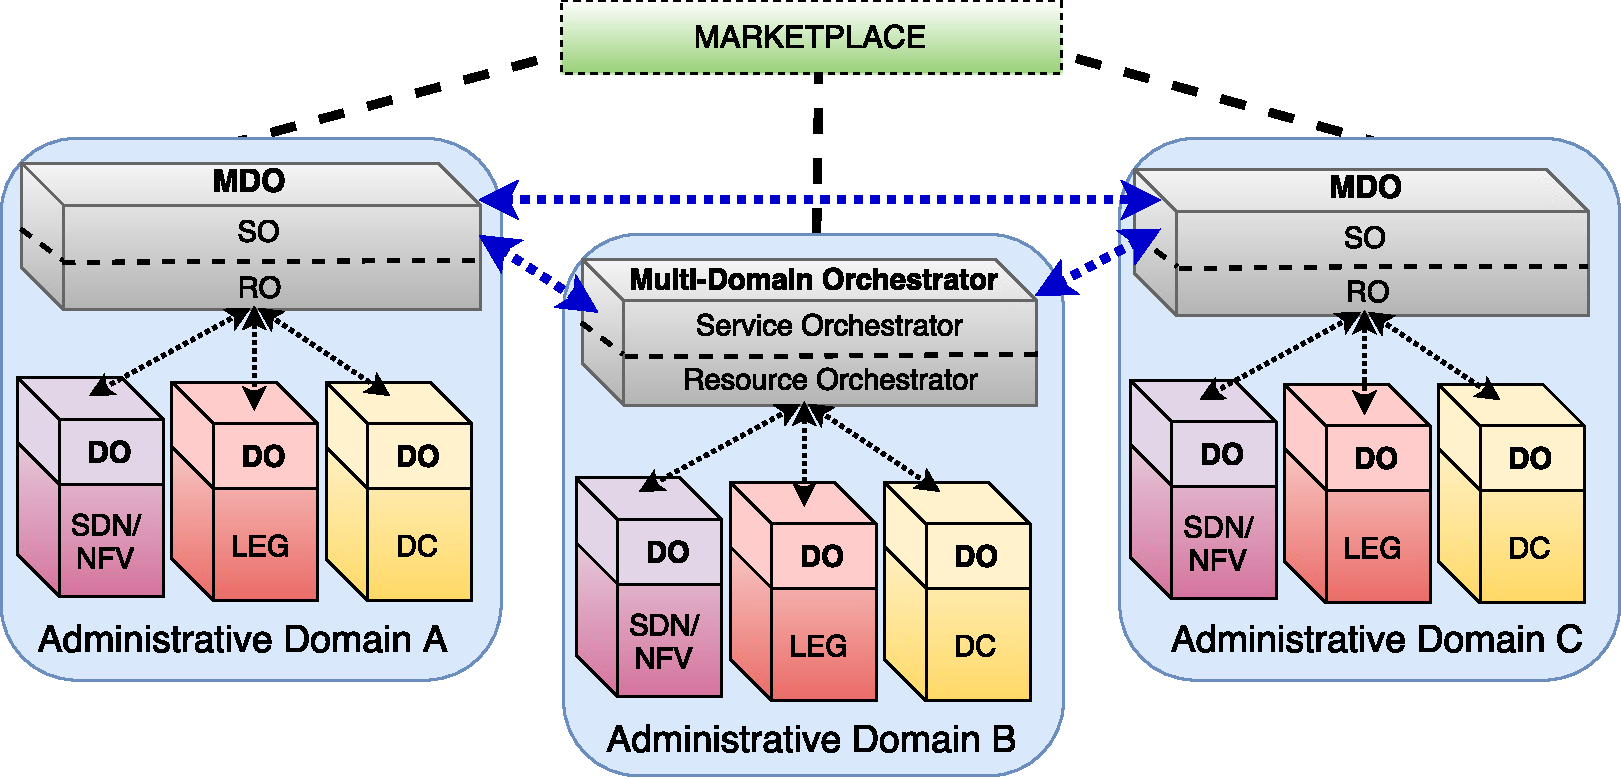
\includegraphics[scale=.6]{Figures/01_Introduction/nso}
    \caption{High-level reference model to illustrate the scope of \acrfull{nso} in single-domain and multi-domain environment. The \gls{nso}  need to have an overview of entire environment to compose the service mainly if it uses resources of different domains.}
    \label{mdo}
\end{figure*}
%a clear definition of \gls{nso}, standardization outcomes, research projects, related frameworks, application scenarios, and challenges.

%The \gls{mdo} exposes the available services to the marketplace. The marketplace allows Service Providers to purchase network services from \acrlongpl{mdo} and offers them to their customers even though the services are composed of resources from other domains.

%Marketplace allows SPs to purchase VNFs from software developers in order to compose NS and offer them to their customers, including SLA management, accounting and billing features and the corresponding interfaces with Service orchestrator.

%The main objective of this paper is to survey on network service orchestration in current context and both single and multi-domain environments. It aims also provide a comprehensive understanding of this new scenarios, its related technologies, as well as the main issues that related with the standardization process. 

%We propose the best of our vision on NSO in this work.


\noindent \textbf{Survey Organization.}  The survey is organized as depicted in Figure~\ref{org}. Section~\ref{sec:background} presents essential background and key technologies related to network service orchestration: Cloud computing, \gls{sdn}, \gls{nfv}, historical overview of orchestration, and the relationship between all mentioned technologies. Section~\ref{sec:scneario} outlines four potential scenarios to illustrate the \gls{nso} in practice. Concepts, functions, scope, and an NSO taxonomy split into seven key aspects are presented in Section~\ref{sec:nso}. Section~\ref{sec:stand} focuses on the standardization outcomes produced by nine important organizations,   whereas Section~\ref{sec:project} covers six major research projects around \gls{nso}. Section~\ref{sec:proj} provides an overview of ten open source solutions and some commercial initiatives.  The discussion in Section~\ref{sec:challenge} points to six groups of open challenges and research opportunities. Finally, Section~\ref{sec:Conclusion} concludes the survey.

%%%%%% Main contributions %%%%%%
% Historical review of term orchestration
% Overview about definition of orchestration in various organizations and works
% Definition clear about Network Service Orchestration 
%%% Relation between orch, management and automation
%%% Its different functions: Service Orch, Lifecycle Orch and Resource Orch.
%%% Difference and definition about Lifecycle and workflow.  
% Taxonomy
% Main outcomes of standardization entities related to NSO
% Approach research projects and the aspects NSO that they address 
% Point the solutions that implement concepts of NSO.